\documentclass[10pt]{article}
\usepackage{amsmath} 
\usepackage{fontspec}
\usepackage[a4paper, margin=12mm]{geometry}
\usepackage{graphicx}
\usepackage{titlesec}
\usepackage{amsmath}
\usepackage{fancyhdr}
\usepackage{amsmath}
\usepackage{datetime}
\usepackage[hidelinks]{hyperref}
\usepackage[utf8]{inputenc}
\usepackage{booktabs}

\setmainfont{Arial}
\setmainfont[NFSSFamily=dayrom]{Arial}
\graphicspath{ {./images/} }

\DeclareSymbolFont{digits}{TU}{dayrom}{m}{n}
\AtBeginDocument{
	\DeclareMathSymbol{0}{\mathalpha}{digits}{`0}
	\DeclareMathSymbol{1}{\mathalpha}{digits}{`1}
	\DeclareMathSymbol{2}{\mathalpha}{digits}{`2}
	\DeclareMathSymbol{3}{\mathalpha}{digits}{`3}
	\DeclareMathSymbol{4}{\mathalpha}{digits}{`4}
	\DeclareMathSymbol{5}{\mathalpha}{digits}{`5}
	\DeclareMathSymbol{6}{\mathalpha}{digits}{`6}
	\DeclareMathSymbol{7}{\mathalpha}{digits}{`7}
	\DeclareMathSymbol{8}{\mathalpha}{digits}{`8}
	\DeclareMathSymbol{9}{\mathalpha}{digits}{`9}
}

% subsubsubsection
\titleclass{\subsubsubsection}{straight}[\subsection]
\newcounter{subsubsubsection}[subsubsection]
\renewcommand\thesubsubsubsection{\thesubsubsection.\arabic{subsubsubsection}}
\renewcommand\theparagraph{\thesubsubsubsection.\arabic{paragraph}} % optional; useful if paragraphs are to be numbered

\titleformat{\subsubsubsection}
{\normalfont\normalsize\bfseries}{\thesubsubsubsection}{1em}{}
\titlespacing*{\subsubsubsection}
{0pt}{3.25ex plus 1ex minus .2ex}{1.5ex plus .2ex}

\makeatletter
\renewcommand\paragraph{\@startsection{paragraph}{5}{\z@}%
	{3.25ex \@plus1ex \@minus.2ex}%
	{-1em}%
	{\normalfont\normalsize\bfseries}}
\renewcommand\subparagraph{\@startsection{subparagraph}{6}{\parindent}%
	{3.25ex \@plus1ex \@minus .2ex}%
	{-1em}%
	{\normalfont\normalsize\bfseries}}
\def\toclevel@subsubsubsection{4}
\def\toclevel@paragraph{5}
%\def\toclevel@paragraph{6}
\def\toclevel@subparagraph{6}
\def\l@subsubsubsection{\@dottedtocline{4}{7em}{4.5em}}
\def\l@paragraph{\@dottedtocline{5}{10em}{5em}}
\def\l@subparagraph{\@dottedtocline{6}{14em}{6em}}
\makeatother

\setcounter{secnumdepth}{4}
\setcounter{tocdepth}{4}


\hypersetup{
	colorlinks=true,
	urlcolor=cyan,
}

% Footer-Einstellungen
\newdateformat{mydate}{\twodigit{\THEDAY}.\twodigit{\THEMONTH}.\THEYEAR}
\mydate
\pagestyle{fancy}
\fancyhf{} % Löscht alle Kopf- und Fusszeilen
\fancyfoot[C]{\thepage\ -\ \today\ \copyright\ Bastian\ Kind,\ James\ Binks,\ Mark\ Matkovic\ und\ David\ Hafner} % Setzt den Foote

\title{DFB Entdecker App}
\author{Bastian Kind, James Binks, Mark Matkovic und David Hafner}

\begin{document}
	\maketitle
	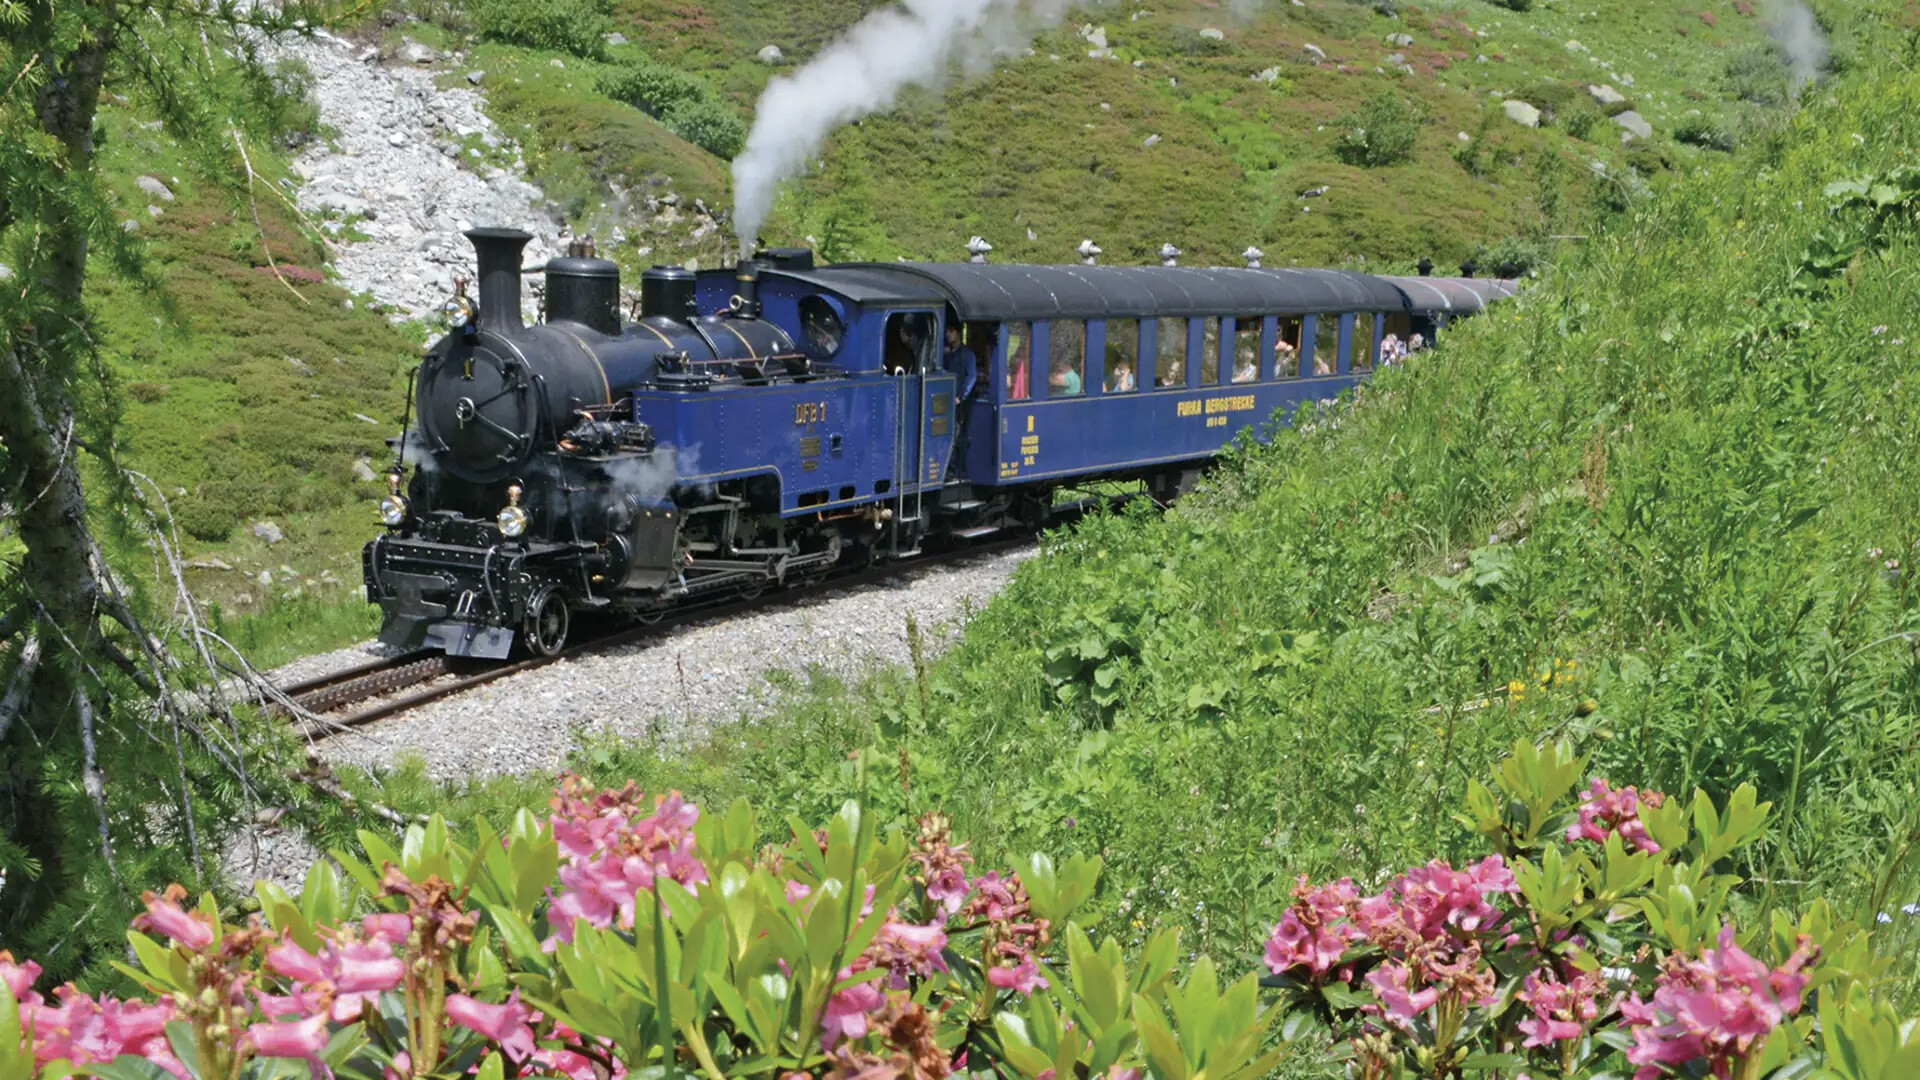
\includegraphics[width=17.5cm]{title}
	\pagebreak
	\tableofcontents
	\pagebreak
	\section{Band A}
	\subsection{Anforderungsanalyse}
	\subsubsection[Wer]{Wer benutzt die App?}
	\begin{itemize}
		\item Familien mit Kindern (z.\,B. als Freizeit-Ausflug)
		\item Rentner / ältere Menschen (Interesse an Geschichte und Eisenbahn)
		\item Erwachsene allgemein (z.\,B. Eisenbahnbegeisterte, Touristen)
		\item Schulklassen (für interaktive, spielerische Lernmöglichkeiten)
	\end{itemize}
	\subsubsection[Wo]{Wo wird die App verwendet?}
	\begin{itemize}
		\item Entlang der Furka-Bergstrecke, einer historischen Dampfbahnstrecke
		\item Draussen (z.B. auf Bahnhöfen, an Brücken, bei Aussichtspunkten)
		\item Oft ohne Mobilfunknetz -> App muss offlinefähig sein
		\item Unterwegs mit dem Zug oder zu Fuss an Haltepunkten
	\end{itemize}
	\subsubsection[Was]{Was muss die App können?}
	\begin{itemize}
		\item QR-Codes an Infopunkten scannen -> Inhalte anzeigen (Text, Bilder, Videos, Audio)
		\item Karte mit GPS nutzen -> aktuelle Position und nahegelegene Punkte anzeigen
		\item Quiz- oder Rätsel-Funktion -> spielerisches Lernen
		\item Tagebuch- oder Sammelfunktion («Meine liebsten Sehenswürdigkeiten»)
		\item Inhalte in mehreren Sprachen (D/E/F/I), evtl. auch einfache Sprache
		\item Inhalte offline verfügbar
		\item Datenschutzkonform -> keine Registrierung, keine Standortüberwachung / Standort wird nicht gespeichert
	\end{itemize}
	\subsubsection[Womit]{Technische Rahmenbedingungen}
	\begin{itemize}
		\item Smartphone oder Tablet, Android und iOS (Dynamisch)
		\item Ressourcenschonendes Design (damit es auch auf älteren Geräten läuft)
		\item App soll Inhalte aus CMS (z.\,B. Texte, Medien) beziehen
		\item Kein Internet nötig unterwegs (alle Inhalte offline verfügbar)
		\item Barrierefreiheit: Vorlesefunktion, grosse Schrift, starke Kontraste
	\end{itemize}
	\subsubsection[Verbesserungen]{Verbesserungen}
	\begin{itemize}
		\item Wir könnten die Benutzergruppen noch genauer unterteilen. Z.\,B. nach technischen Kentnissen, Alter oder ob die Nutzer einheimische oder Touristen sind.
		\item Wir könnten konkrete Anforderungen für barrierefreies Design formulieren. Z.\,B. Schriftgrössen, Bedienung mit Screenreader, Kontraste
		\item Wir könnten die Datenschutzanforderungen genauer definieren. Z.\,B. Wie werden die GPS Daten verarbeitet?
		%\item \textbf{Gamification weiterdenken:} Die Rätsel- und Sammelfunktionen könnten mit Badges, Levels oder Belohnungen erweitert werden, um die Motivation zu steigern.
	\end{itemize}
	\pagebreak
	\subsection{Vorgehensmodell}
	\subsubsection{Wahl des Modells}
	% Erklärung, welches Vorgehensmodell gewählt wurde (z. B. Design Thinking, User Centered Design) und warum
	Wir haben das Vorgehensmodell Design Thinking gewählt, da es gut zu unserem Projekt passt. Es ist benutzerorientiert und iterativ. Es gibt viel Nutzerfeedback und das Endprodukt ist das, was der Nutzer will.\\
	So können wir sicherstellen, dass wir uns nicht in Details verlieren, die dem Nutzer schlussendlich wenig nützen. Wir werden uns so besser auf die Wünsche und die Bedürfnisse des Nutzers konzentrieren können.
	\subsubsection{Phasen des Modells}
	% Beschreibung der einzelnen Phasen des gewählten Modells mit kurzer Erklärung (z. B. beim Design Thinking: Verstehen, Beobachten, Sichtweise definieren, Ideen finden, Prototyp bauen, Testen)
	Design Thinking hat zwei «Räume». Es gibt den Problemraum und den Lösungsraum. Im Problemraum schaut man die Probleme an.
	\begin{itemize}
		\item Verstehen
		\subitem Als erstes muss man das Umfeld und die Nutzer verstehen.
		\item Beobachten
		\subitem Dann schaut man, wie sich der Nutzer verhält.
		\subitem Was macht der Nutzer, was ist ihm am wichtigsten, womit verbringt er viel Zeit.
		\item Standpunkt definieren
		\subitem Die gewonnen Erkenntnisse muss man dann aufschreiben und nach Wichtigkeit filtern oder sortieren.
		\subitem Möglicherweise braucht man noch mehr Informationen und muss nochmals zu einem der beiden vorherigen Schritte zurückgehen.
	\end{itemize}
	Im Lösungsraum überlegt man sich dann Lösungen für die gefundenen Probleme.
	\begin{itemize}
		\item Ideen finden
		\subitem Im ersten Schritt im Lösungsraum überlegt man sich, wie man die Probleme lösen könnte
		\item Prototyp entwickeln
		\subitem Zu diesen Ideen entwickelt man dann einen Prototypen.
		\item Testen
		\subitem Diesen Prototypen testet man dann mit dem Nutzer
		\subitem Mit dem erhaltenen Feedback muss man dann evtl. Zu einem der vorherigen Schritte zurückkeren und Verbesserungen vornehmen.	
	\end{itemize}
	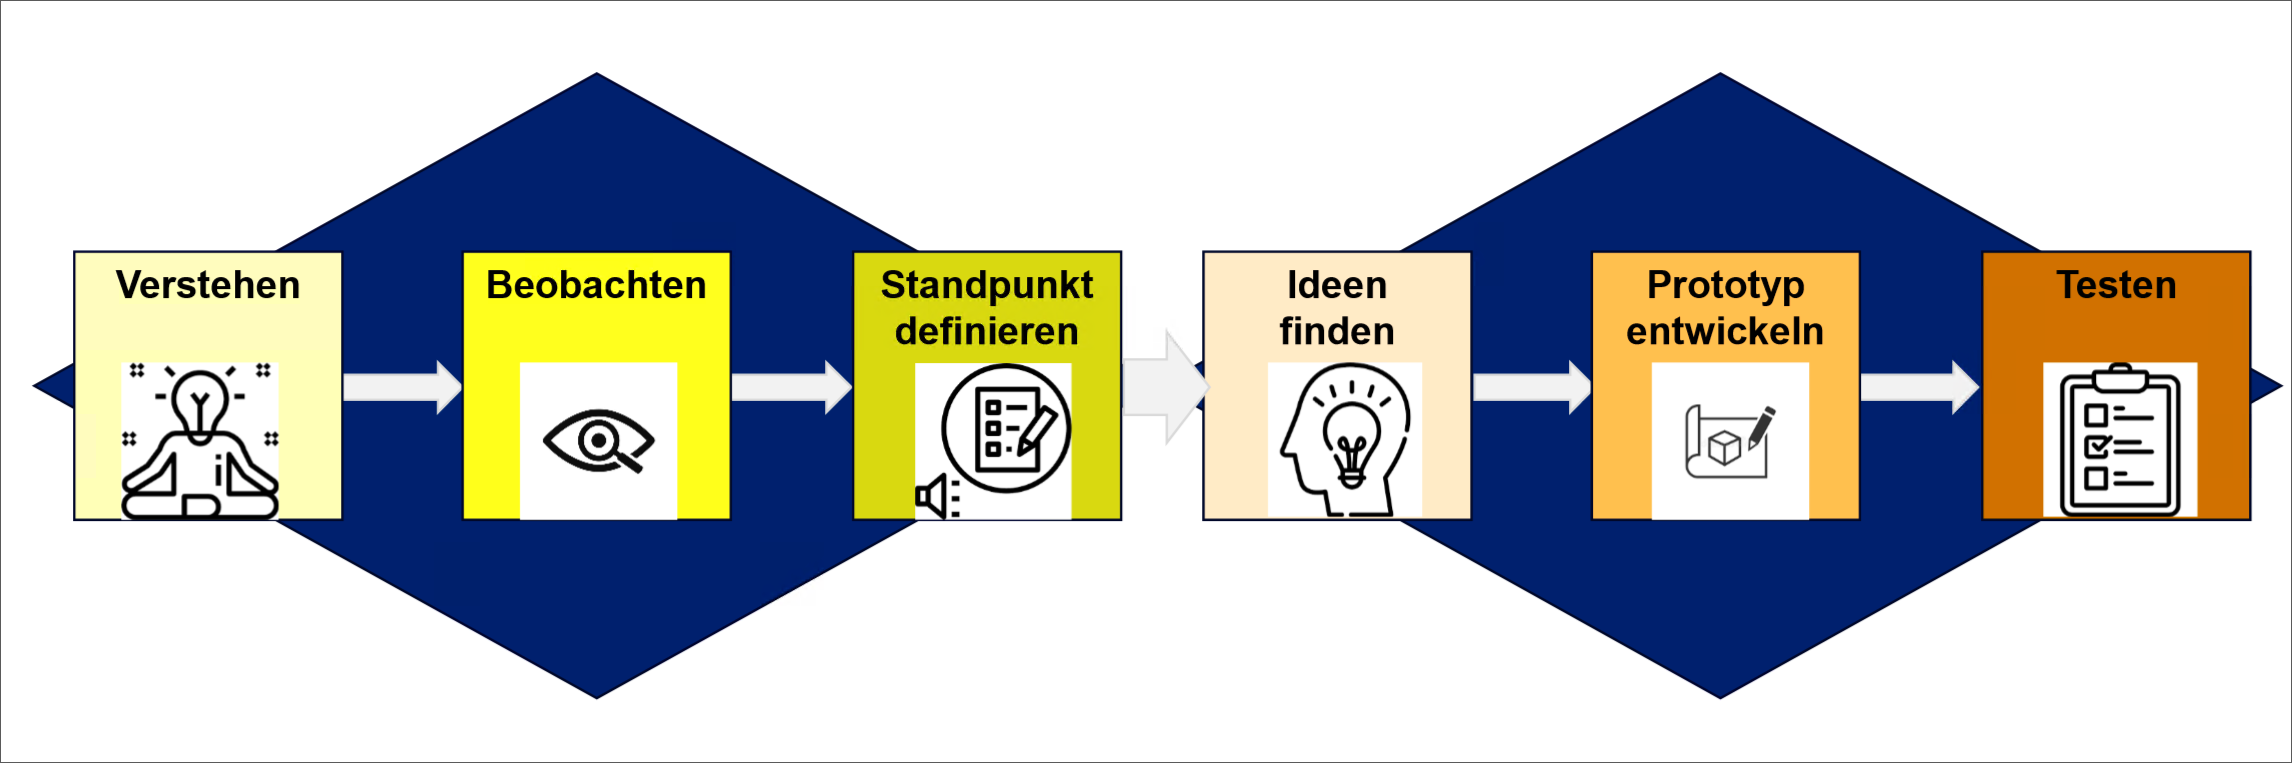
\includegraphics[width=18.6cm]{DesignThinking}
	\pagebreak
	\subsection{Nutzungskontext}
	
	\subsubsection{Methoden zur Kontextanalyse}
	
	\begin{itemize}
		\item Beobachtungen vor Ort entlang der Strecke
		\item Interviews mit Besuchern
		\item Analyse von Bewertungen der DFB
		\item Elektronische Umfragen
	\end{itemize}
	
	\subsubsection{Analyseergebnisse}
	\begin{itemize}
		\item Die Strecke liegt in einem abgelegenen Berggebiet – Mobilfunknetz ist nur teilweise verfügbar.
		\item Die Nutzung erfolgt draussen: an Bahnhöfen, Aussichtspunkten, Infotafeln oder im Zug.
		\item Nutzer sind häufig zu Fuss unterwegs und haben nur kurz Zeit für Interaktion.
		\item Zielgruppe ist sehr durchmischt: Kinder, Erwachsene, Senioren, Touristen, Schulklassen.
		\item Viele Nutzer wünschen sich eine spielerische, leicht verständliche und multilinguale Erfahrung. (Viedos und illustration)
	\end{itemize}
	
	\subsubsection{Schlussfolgerungen für die App}
	\begin{itemize}
		\item Die App muss vollständig offlinefähig sein.
		\item Eine einfache Bedienung ist nötig, besonders für Kinder und ältere Menschen.
		\item Ein intuitives und zweckdienliches Design
		\item Barrierefreiheit ist wichtig: grosse Schrift, kontrastreiche Farben, Vorlesefunktion.
		\item Inhalte müssen mehrsprachig verfügbar sein (De/En/Fr/It), mit vereinfachtem Deutsch für Kinder.
		\item Zusätzliche detailliertere informationen für enthusiasten.
		\item Die App sollte schnell Informationen liefern, da Nutzer meist unterwegs oder in Bewegung sind.
	\end{itemize}
	\pagebreak
	\subsection{Benutzereigenschaften}
	\subsubsection{Warum werden Benutzereigenschaften erfasst}
	\begin{itemize}
		\item Wir erfassen Benutzereigenschaften, damit wir uns besser vorstellen können, welche Bedürfnisse die Benutzer haben und wie sie sich verhalten.
		\item Wenn wir die Ziele der Benutzer erfassen, also was die Benutzer auf der App wollen, können wir schauen, dass sie ihre Ziele einfacher erreichen können.\
		\item Die Benutzerbedürfnisse erfassen wir, damit wir diese in den Vordergrund stellen können. So priorisieren wir das, was den Nutzern am wichtigsten ist.
	\end{itemize}
	\subsubsection{Personas}
	\begin{itemize}
		\item \textbf{Familie Müller} (Eltern 40/38, Kinder 8/12)
		\subitem \textbf{Hintergrund}: Tagesausflug mit Kindern, wenig technikaffin
		\subitem \textbf{Ziele}: 
		\begin{itemize}
			\item Schneller Zugang zu kindgerechten Inhalten
			\item Offline-Karten für Wanderwege
			\item Spielerische Quiz-Funktion
		\end{itemize}
		\subitem \textbf{Schmerzpunkte}: 
		\begin{itemize}
			\item Komplexe Menüs
			\item Lange Ladezeiten ohne Netz
		\end{itemize}
		
		\item \textbf{Hans Meier} (65, Eisenbahn-Enthusiast)
		\subitem \textbf{Hintergrund}: Pensioniert, historisch interessiert
		\subitem \textbf{Ziele}: 
		\begin{itemize}
			\item Technische Details zu Lokomotiven
			\item Historische Vergleichsbilder
			\item Präzise GPS-Positionsanzeige
		\end{itemize}
		\subitem \textbf{Schmerzpunkte}: 
		\begin{itemize}
			\item Kleine Schriftgrössen
			\item Fehlende Tiefeninformationen
		\end{itemize}
		
		\item \textbf{Laura Bianchi} (28, internationale Touristin)
		\subitem \textbf{Hintergrund}: Backpacking in der Schweiz
		\subitem \textbf{Ziele}: 
		\begin{itemize}
			\item Mehrsprachige Audio-Guides (EN/IT)
			\item Social-Media-Integration
			\item Datensparsame Nutzung
		\end{itemize}
		\subitem \textbf{Schmerzpunkte}: 
		\begin{itemize}
			\item Hoher Datenverbrauch
			\item Unklare Wegführung
		\end{itemize}
		
		\item \textbf{Teenager Alex} (15, lokaler Jugendlicher)
		\subitem \textbf{Hintergrund}: Nutzt App mit Schulkameraden
		\subitem \textbf{Ziele}: 
		\begin{itemize}
			\item Gamification (Badges sammeln)
			\item Foto-Challenges mit Hashtags
			\item Schnelles Teilen von Entdeckungen
		\end{itemize}
		\subitem \textbf{Design-Implikation}: 
		\begin{itemize}
			\item Einfache Social-Media-Buttons
			\item Visuell ansprechende Achievements
		\end{itemize}
	\end{itemize}
	\subsubsection{Verbesserungen}
	\begin{itemize}
		\item \textbf{Familie Müller (Kinder-Modus)}
		\subitem \textbf{Problem}: 
		\begin{itemize}
			\item Quiz-Fragen nicht altersgerecht differenziert
			\item Eltern/Kinder nutzen dieselbe Oberfläche
		\end{itemize}
		\subitem \textbf{Anpassung}: 
		\begin{itemize}
			\item „Kinder-Modus“ mit vereinfachten Fragen + Emojis
			\item Eltern können Modus per Passcode sperren
		\end{itemize}
		\subitem \textbf{Design-Implikation}: 
		\begin{itemize}
			\item Toggle-Schalter „Kindermodus“ in der Navigation
			\item Visuelle Icons statt Textbuttons
		\end{itemize}
		
		\item \textbf{Hans Meier (Schriftgrösse)}
		\subitem \textbf{Problem}: 
		\begin{itemize}
			\item Standard-Schrift für Outdoor-Nutzung zu klein
			\item Keine Anpassungsmöglichkeiten
		\end{itemize}
		\subitem \textbf{Anpassung}: 
		\begin{itemize}
			\item Schriftgrössen-Slider (100\%–200\%)
			\item Kontrastmodus für Sonnenlicht
		\end{itemize}
		\subitem \textbf{Design-Implikation}: 
		\begin{itemize}
			\item Dynamische UI-Anpassung aller Textelemente
			\item Persistente Einstellung über App-Neustart
		\end{itemize}
		
		\item \textbf{Laura Bianchi (Sprachumschaltung)}
		\subitem \textbf{Problem}: 
		\begin{itemize}
			\item Sprachwechsel erfordert 4 Klicks
			\item Keine Gerätesprachen-Erkennung
		\end{itemize}
		\subitem \textbf{Anpassung}: 
		\begin{itemize}
			\item Automatische Sprachwahl basierend auf Gerät
			\item Sprach-Icon in Top-Leiste
		\end{itemize}
		\subitem \textbf{Design-Implikation}: 
		\begin{itemize}
			\item Dropdown-Menü mit Flaggen-Icons
			\item Sprachwechsel ohne App-Neustart
		\end{itemize}
		
		\item \textbf{Teenager Alex (Gamification)}
		\subitem \textbf{Problem}: 
		\begin{itemize}
			\item Achievements motivieren nicht nachhaltig
			\item Keine Social-Media-Verlinkung
		\end{itemize}
		\subitem \textbf{Anpassung}: 
		\begin{itemize}
			\item „Badge-System“ mit Leveln (Bronze–Platin)
			\item Direktes Teilen auf Instagram/TikTok
		\end{itemize}
		\subitem \textbf{Design-Implikation}: 
		\begin{itemize}
			\item Progress-Bar im Profil-Bereich
			\item Ein-Klick-Share-Buttons
		\end{itemize}
	\end{itemize}
	
	\subsubsection{Priorisierung der Anpassungen}
	\begin{center}
		\begin{tabular}{|l|l|l|}
			\hline
			\textbf{Anpassung} & \textbf{Relevanz} & \textbf{Aufwand} \\ 
			\hline
			Schriftgrössen-Slider & Hoch & Niedrig \\
			Kinder-Modus & Mittel & Mittel \\
			Automatische Sprachwahl & Hoch & Hoch \\
			Badge-System & Mittel & Hoch \\
			\hline
		\end{tabular}
	\end{center}
	
	\textit{Begründung: Schriftgrössen-Slider wurde priorisiert, da essenziell für Barrierefreiheit und einfach umsetzbar.}
	\pagebreak
	\subsection{Nutzungsanforderungen}
	\subsubsection{Einleitung}
	Die Spezifikation der Nutzungsanforderungen ermöglicht es, die Bedürfnisse der Nutzer in konkrete To-Dos umzuwandeln.\\
	Dafür verwenden wir User Stories, die typische Nutzungssituationen beschreiben.
	\subsubsection{User Stories}
	\begin{itemize}
		\item Als Familienvater möchte ich eine Simple und intuitive Darstellung, so dass meine Kinder alles verstehen können.
		\item Ich als Senior möchte eine Grosse und klare Schrift, so dass ich diese gut lesen kann.
		\item Als Tourist möchte ich eine Karte mit GPS-Ortung nutzen können, um interessante Punkte entlang der Strecke zu finden.
		\item Als Kind möchte ich Quizfragen beantworten, damit ich spielerisch etwas über die Eisenbahn lernen kann.
		\item Als Lehrperson möchte ich die App offline nutzen können, damit ich mit der Klasse auch ohne Netz arbeiten kann.
	\end{itemize}
	
	\subsubsection{Priorisierung}
	\begin{itemize}
		\item \textbf{Must-Have}: QR-Scan, Offline-Funktion, mehrsprachige Inhalte, intuitive Bedienung
		\item \textbf{Should-Have}: Quizfunktion, GPS-Karte, Tagebuch/Sammelmodus
		\item \textbf{Could-Have}: Dialekte, individuelle Empfehlungen, erweiterte Suchfunktion
	\end{itemize}
	
	\pagebreak
	
	\section{Band B}
	\subsection{Grundsätze der Dialoggestaltung verstehen}
	\subsubsection[Konzept der Gebrauchs Tauglichkeit]{Das Konzept der Gebrauchstauglichkeit}
	\begin{itemize}
		\item Effektivität: Wie genau und vollständig können Nutzer ihr Ziel mit der App erreichen. Gibt es Errors oder sind Informationen Unvollständig? Bsp. herausfinden wo sie im park sind oder welche informationen mit einem Ausstellungsstück in verbindung stehen.
		
		\item Effizienz: Wie effizient kommen die Nutzer in der App and die erwünschten Informationen. Braucht es viele unnötige clicks, sind die Seiten logisch kategorisiert, sind die Seiten zweckmässig angeschrieben, gibt es eine Suchfunktion, etc.
		
		\item Zufriedenstellung: Ist der Nutzer nach der Interaktion mit der App zufrieden. Hat er alles gefunden was gesucht wurde und möchte er die App wieder verwenden oder ist er frustriert weil nichts dort war wo es sein sollte.
	\end{itemize}
	\subsubsection [Benuzterschnitstellen und Interaktonsprinzipien erkläret] {Benutzerschnittstellen und Interaktonsprinzipien erklärt}
	\begin{itemize}
		\item \textbf{Was ist eine Benutzerschnittstelle}
		\\ Eine Benutzerschnittstelle ist der Punkt wo sich Mensch und Maschiene treffen. Eine der Simpelsten Versionen davon ist der Lichtschalter. Einmal drauf drücken und die Maschiene (das Licht) Reagiert auf den Menschlichen Input und ist somit die Simpelste Benutzerschnittstelle.
		
		In Unserem fall ist für uns eine Benutzerschnittstelle ein User Interface/ Die GUI unser Applikation. Dort werdenalli Inputs der User getätigt und unsererer Applikation weitergeleitet.
		
		\item \textbf{Was sind Interaktionsprinzipien}
		\\ Interaktonsprinzipien sind nach ISO 9241-110 normungen für die Wichtigsten Eigenschafte der Benutzerschnitstellen und besteht aus diesen 7 Prinzipien welche mit Beispiel eines Standard Webshops erklärt werden.
		\begin{itemize}
			\item \textbf{Aufgabenangemessenheit}
			\\ Es gibt an wie gut die Webseite ihren zweck werfüllt. In einem Onlineshop wäre es ob man seine Einkäufe Problemlos in den Warenkorb bewegen kann ohne das es Errors gibt.
			\item \textbf{Selbstbeschreibungsfähigkeit}
			\\ Es gibt an wie intuitive die Webseite gestaltet ist. Bsp sollen Symbole verwendet werden um das Suchfenster oder den Warenkorb zu zeigen damit nicht für alles eine Lange erklärung gebraucht wird.
			\item \textbf{Erwartungskonformität}
			\\ Bei Manche arten von Webseiten wie Onlineshops gibt es eine gewisse erwartungsstellung an das Layout der Webseit. Bsp. es gibt vorgeschlagen produkte, Banner mit Rabatt aktionen und ein suchfenster.
			\item \textbf{Erlernbarkeit}
			\\ Besagt das eine Seite schnell erlernbar sein sollte und man nicht dafür zuerst eine Weiterbildung abschleissen muss. Bei einem Onlineshop geht es hier hauptsächlich um die Intuitive gestaltung
			\item \textbf{Steuerbarkeit}
			\\ Besagt das der Nutzer immer in kontrolle sein sollte. Der Nutzer soollte immer wisse wo er ist und wie man zurück kommt. Bsp. eie gute Navbar mit einem Homebutton
			\item \textbf{Robustheit}
			\\ Besagt das es inputsicherheit gibt damit der Nutzer möglichst wenig Fehler machen kann.
			\item \textbf{Benutzer:innen-Bindung}
			\\ Besagt das es Feedback möglichkeiten von den Nutzern gibt.
		\end{itemize}
	\end{itemize}
	\subsubsection[geforderte Benutzerschnittstelle]{geforderte Benutzerschnittstelle}
	Eine der Meist gebrauchten Benutzerschnittstellen wird die Hauptseite sein wenn man versucht die Seite zu einem Bestimmten ort zu finden. Dies kann über das Manuelle Navigieren der Seiten, der eingebauten Suchfunktion oder vor Ort mit dem Scannen eines QR codes gemacht werden.
	\begin{itemize}
		\item Aufgabenangemessenheit: Es gibt mehrere möglichkeiten an die Gewünschten Informationen zu kommen und limitiert einen nicht bei der Informationsbeschaffug. Bsp. Man könnte sich eine Seite nach der Anderen durchnavigiren und alle umliegenden Informationen auch auffassen. Wenn man aber grade davor steht oder sich spezifisch für eines Interessiert kann man auch nur direkt Relevante schnell finden.
		
		\item Selbstbeschreibungsfähigkeit: Die Hauptseite wird intuitive mit symbolen dargestellt sein (bsp. ein QR-code zum drücken um einen QR-code scannen zu können oder eine Lupe für die Suchfunktion) damit es für alle, auch kleine Kinder, verständlich ist. Es wird auch immer eine Navbar geben welche angibt wo man sich auf der Seite befindet und einen Knopf der dierekt zur Hauptseite zurückführt.
		
		\item Erwartungskonformität: Der fokus der Seite wird immer auf der angabe der Informationen liegen da das der Hauptnutzen für die meisten User sein wird. Es sollten alle wichtigen infos als erstes angezeigt werden und deteilliere infos wie technische deepdives sollte eher am ende oder etwas abseits sein.
		
		\item Erlernbarkeit: Die Erlernbarkeit hängt sehr mit der Selbstbeschgreibungsfähigkeit zusammen und sollte deshalb durch die Intuitive gestaltung der Applikation bereits gewährleistet sein. Wenn für etwas ein Tutorial notwendig sein würde ist es wahrscheinlich schlecht gestaltet oder unnötig kompliziert.
		
		\item Steuerbarkeit: Die Steuerbarkeit wird damit garantiert das keine Automatischen, nicht vom User gepromteten Popups oder Weiterleitungen verwendet werden und der User immer eine Navbar hat die ihm erlaubt zur Hauptseite zurückzukehren und die Parent Seiten der zurzeit angezeigten Seiten zu Erreichen.
		
		\item Robustheit gegen Nutzungsfehler: Das Fehlverwenden des QR-codes und der Seite zu Seite Navigation ist bereits sehr erschwehrt und in der Suchfunktion sollen, falls keine übereinstimmung vorhanden ist, ähnliche sachen angezeigt werden. Überall wo der User sonst einen Input geben kann wird genügend inputsicherheit und selbstbeschreibende Fehlermeldungen implementiert.
		
		\item Benutzer:innen-Bindung: Eine Seite mit mögliche Kontaktionformationen der Personen die die Seite und den Park betreiben damit man Rückmeldungen geben kann. 
		
	\end{itemize}
	\subsection{Benutzerschnittstelle entwerfen}
	\subsection{Interaktionsprinzipien anwenden}
	\subsubsection{Interaktionselemente identifizieren}
	\subsubsubsection{Was sind Interaktionselemente}
	
	Interaktionnselemente sind die verschiedenen teile einer GUI mit welchen der User interagieren kann. Bsp. ein Knopf oder ein Suchfeld. Alles was der User anclicken kann welches etwas auslöst ins ein Interaktionselement.
	
	\subsubsubsection{Beispiel von Interaktionselementen}
	Für unser beispiel verwenden wir die Digitech Webseite, spezifisch die Hauptseite.
	
	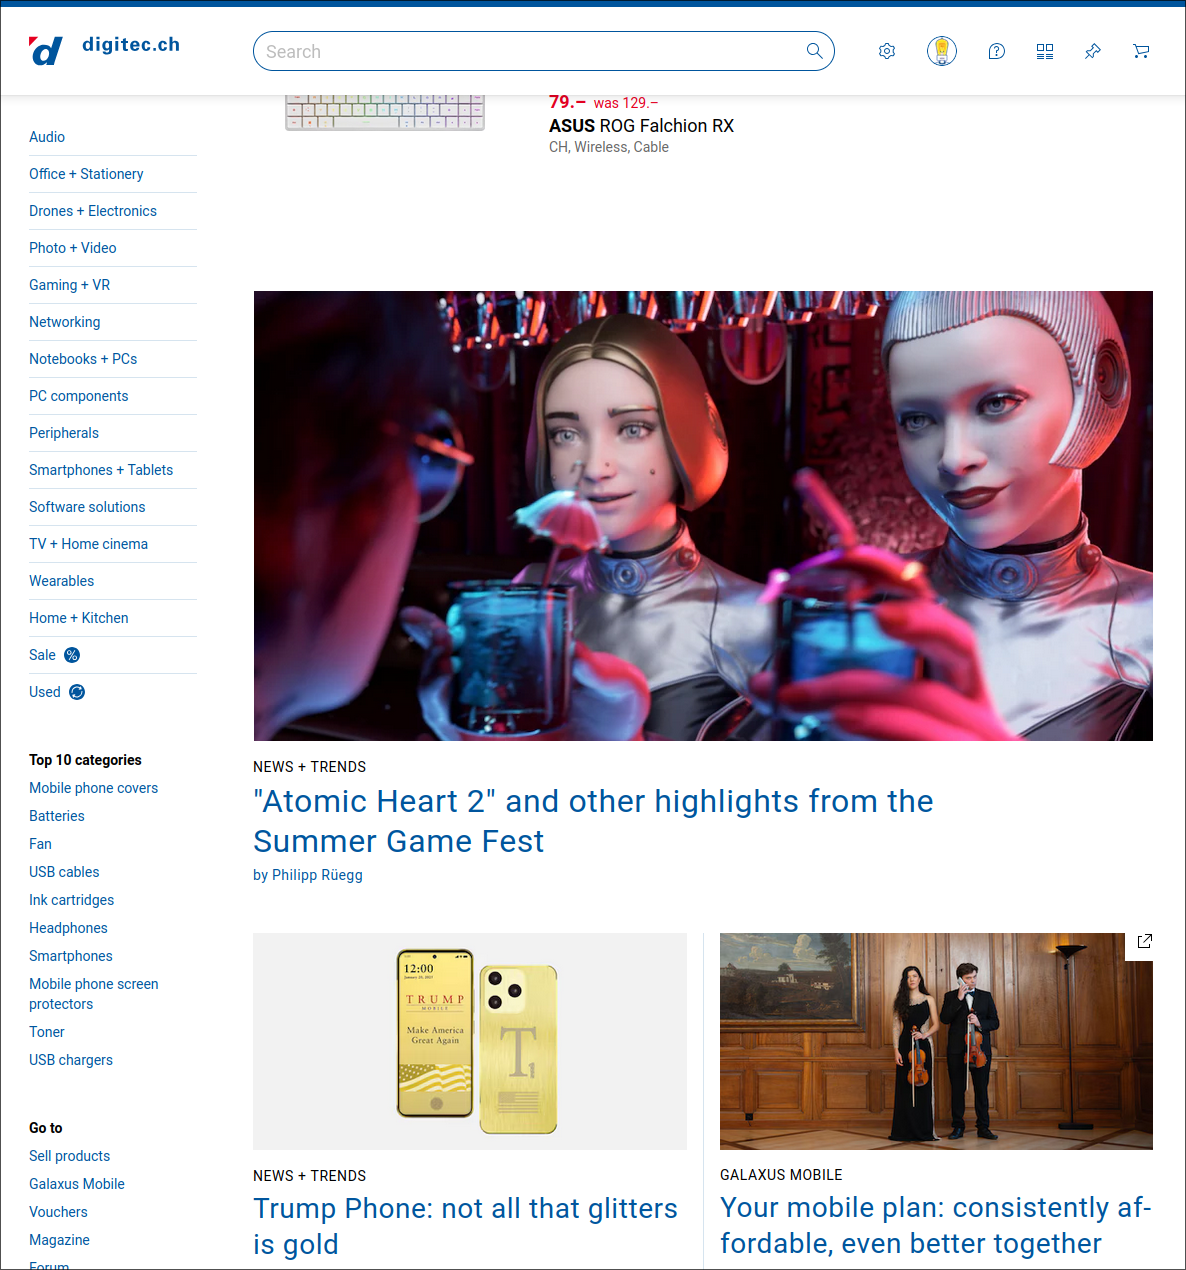
\includegraphics[width=17cm]{DigitechHomepage}\\\\
	
	Interaktionselemente aufgelistet
	\begin{itemize}
		\item Suchfeld:\\
		Das suchfeld ist eines der Zentralen Interaktionselemente Der Webseite. Über diese kann der User spezifische sachen suchen. Das Suchfeld wird fast immer angezeigt damit der User mehr steuerbarkeit hat.
		\item Zentrale Werbung:\\
		Die zentrale Werbung informiert den User über irgendetwas neues. Werbung alleine ist aber kein Interaktionselement, es ist in diesem fall aber eines weil man durch das Clicken auf den Namen oder das Bild des gezeigten Produkts auf dieses weitergeleitet wird.
		\item Seitliche Kategorien auflistung:\\
		An der Seite der Webseite werden alle möglichen Kategorien aufgelistet. Diese sind alles Weiterleitungen zu einem vorgefilterten Suchergebinss und sind deshalb auch Interaktionselemente
		\item Logo als "Home Button":\\
		Ein Logo als ein "Home Button" oder einfach einen Link zur Hauptseite zu verwendin ist heutzutage überall zu erwarten. Es erhöt die Steuerbarkeit der Applikation weil der User immer einen schnellen weg zurück zur Hauptseite hat. Und da es nicht nur ein schönes Bild ist sondern auch eine Funktion hat, die weiterleitung an die Hauptseite, gilt es auch als Interaktionselement.
		\item Konto, Einstellungen, Warenkorb, etc knöpfe:\\
		Diese sind die Simpelsten arten Von Iteraktionselemente. Knöpfe welche genau einen Nutzern erfüllen, in diesem fall weiterleiten an die nötige Seite,< und dies gut machen.
	\end{itemize}
	\subsubsection{Interaktionselemente nach Konventionen verwenden}
	\subsubsubsection{Konventionen der Interaktionselemente}
	\begin{itemize}
		\item Button:\\
		Rechteckig oder abgerundet, beschriftet mit einer Handlungsaufforderung (z. B. „Absenden“).
		\item Hyperlink:\\
		Blauer, unterstrichener Text, der beim Klick eine Seite wechselt.
		\item Checkbox:\\
		Ein kleines Kästchen, das durch einen Klick aktiviert (✓) oder deaktiviert wird.
		\item Radiobutton:\\
		Rundes Auswahlfeld für exklusive Auswahlmöglichkeiten.
		\item Hamburger-Menü:\\
		Drei horizontale Striche für ein aufklappbares Navigationsmenü.
		\item Suchfeld:\\
		Textfeld mit Lupensymbol, Eingabe und Enter oder Klick auf die Lupe löst Suche aus.
		\item Breadcrumb-Navigation:\\
		Hierarchische Anzeige des Navigationspfads.
	\end{itemize}
	\subsubsubsection{Interaktionselemente Anwenden}
	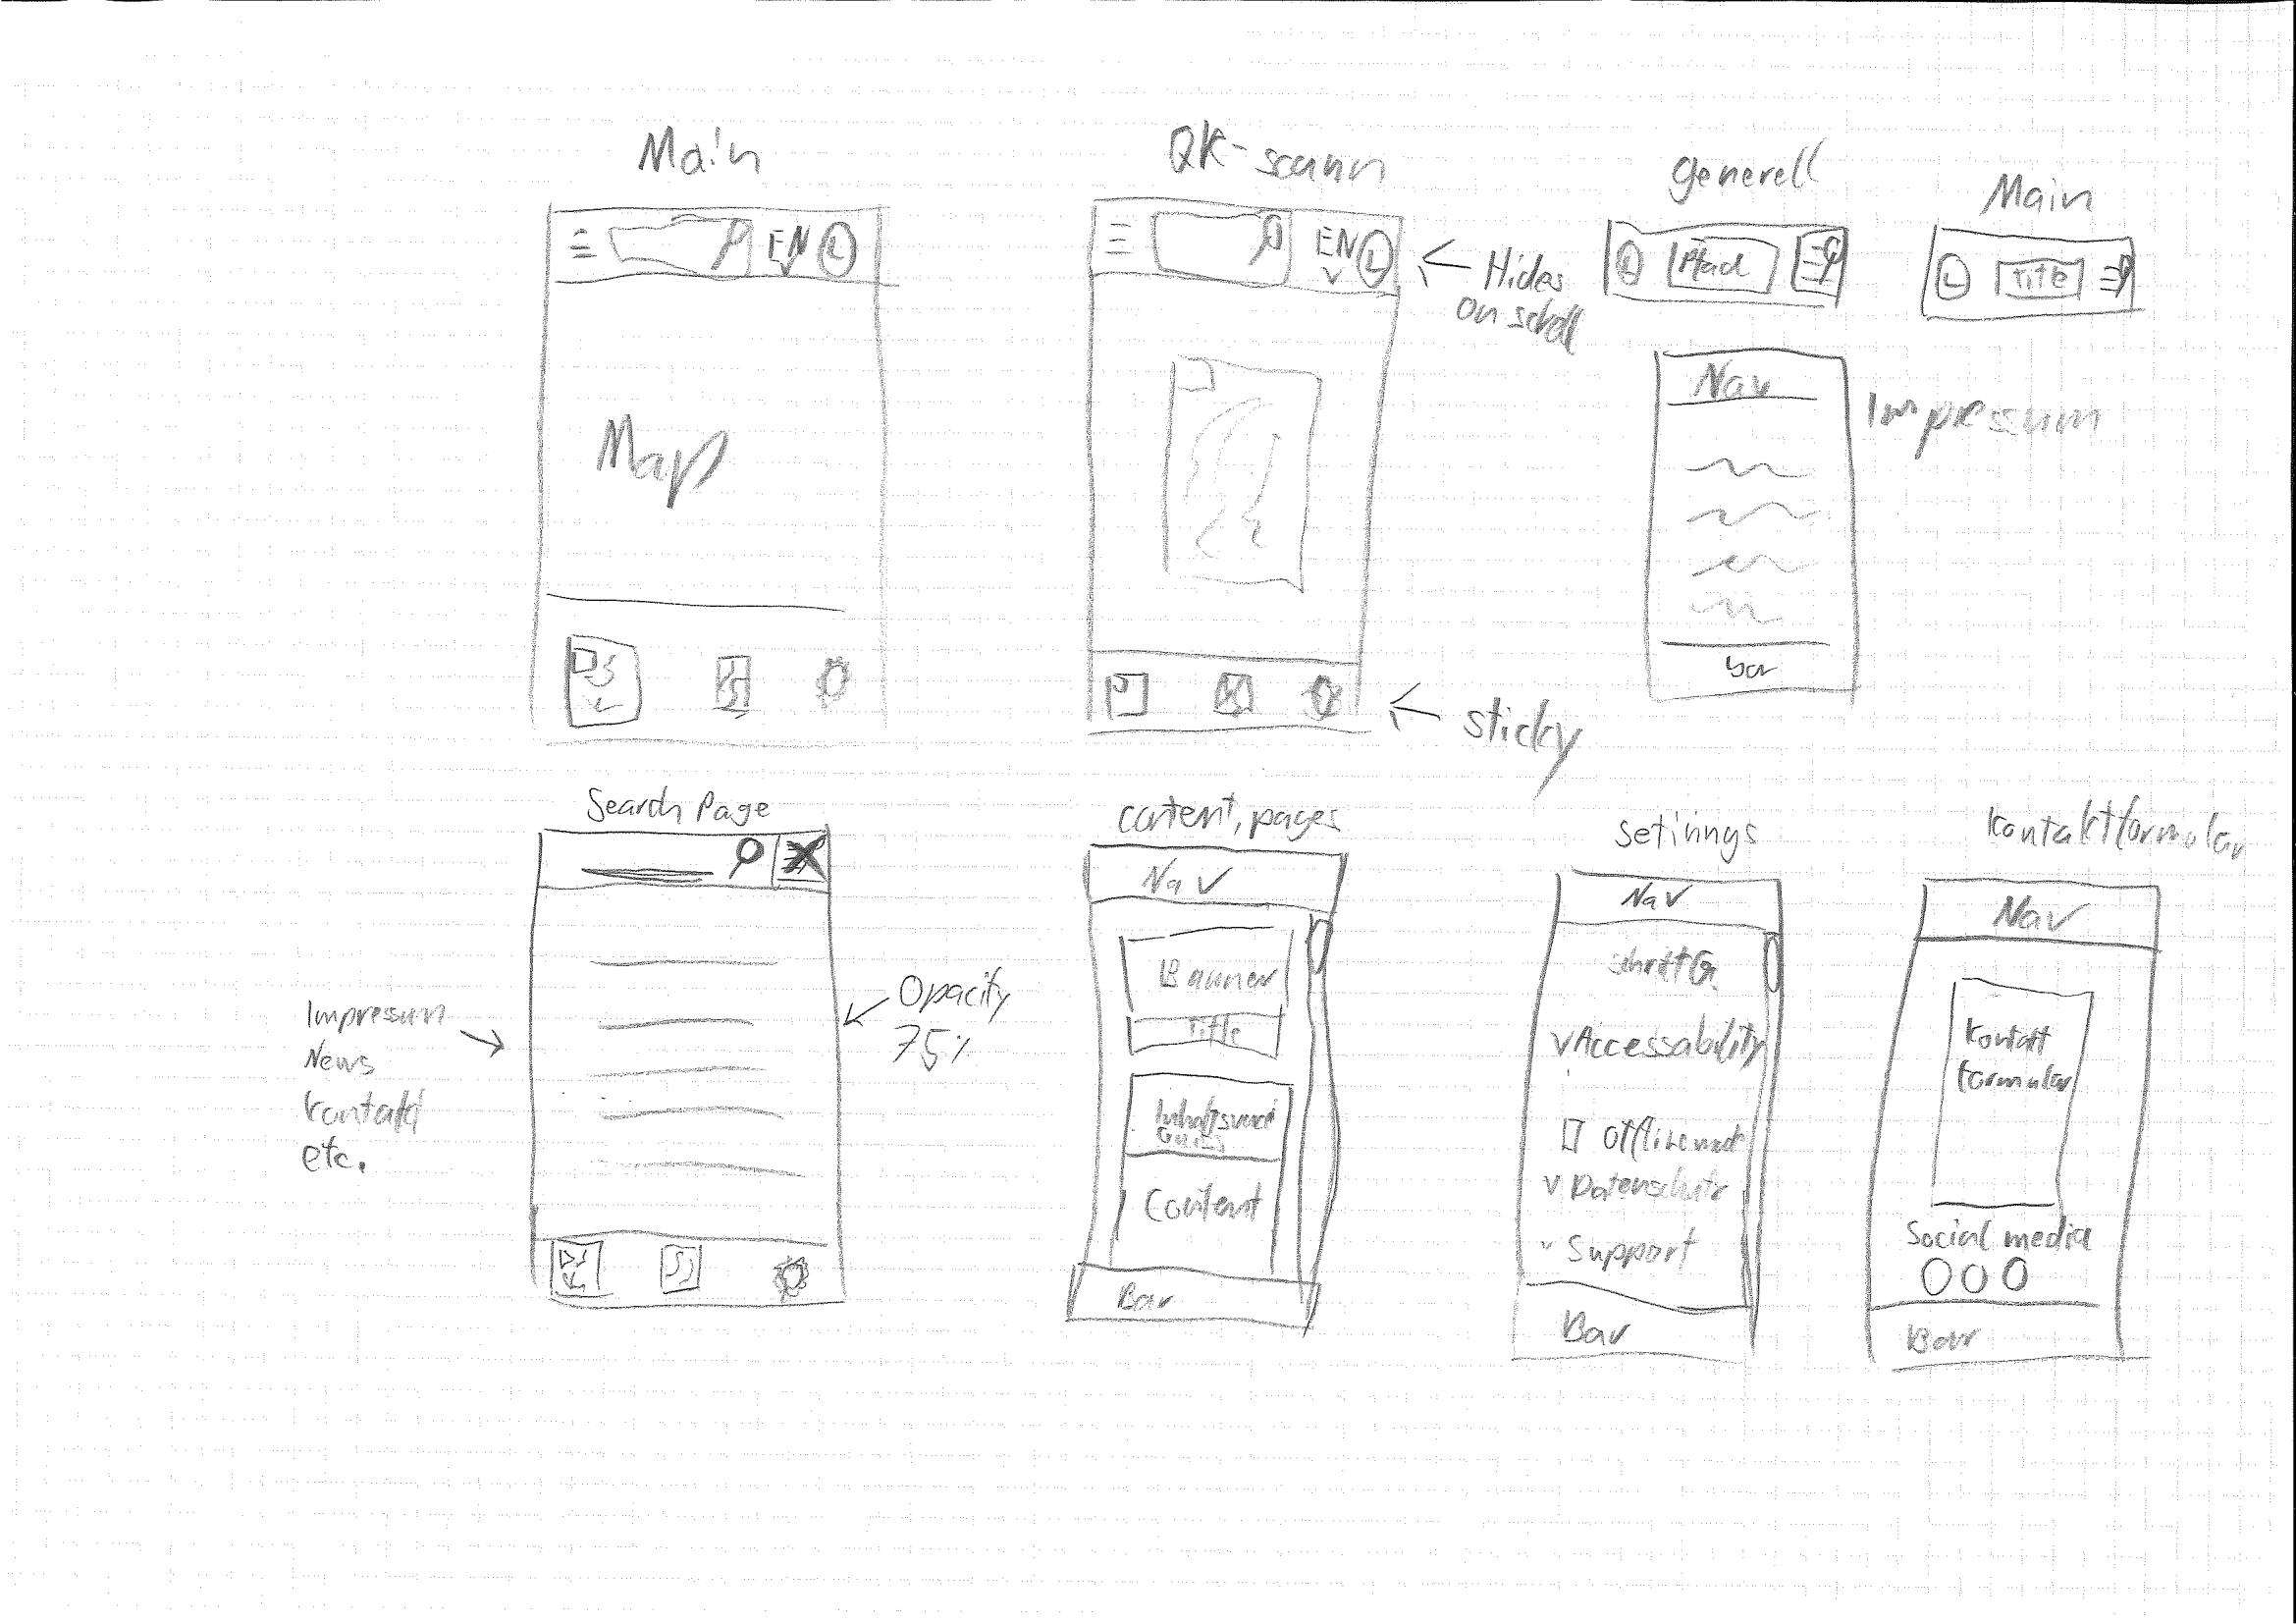
\includegraphics[width=17cm]{scribles-2-1}
	\\Wir legen unseren Fokus auf die Hauptseite hier als Main gekennzeichnet.\\
	Wir starteten mit einer simplen Navbar welche aus 4 Teilen besteht.
	\begin{itemize}
		\item Burgermenu:\\
		Welches eine Seite mit allen möglichen Weiterleitungen zu den Kontaktinformationen, Impressum, feedbackmöglichkeiten, etc. öffnet.
		\item  Suchfeld:\\
		Welches für das suchen der Einzelnen Atraktionen oder Kategorien gebraucht werden kann.
		\item Dropdwon Spracheinstellungen:\\
		Es sollen Deutsch, Englisch, Französich und Italensich zur verfügung stehen.
		\item  Logo:\\
		Zum Schluss fügten wir noch ein Logo welches auch als home Button agieren sollte hinzu.
	\end{itemize}
	Der Haupttil der Seite wird von der Karte des Areals verwendet. Diese Karte sollte interaktiv sein damit man schnell sehen kann wo man ist und wo man hin will.\\
	
	Unten haben wir eien Footer mit drei Knöpfen.
	\begin{itemize}
		\item QR-Code scanner:\\
		Leitet einen weiter auf die QR-Code scanner Seite
		\item  Karte:\\
		In der Mitte und als standard ausgewählt ist die Karte.
		\item Einstellungen:\\
		Alle relevanten einstellungen für die Applikation, wie Darkmode oder ein Screenreader.
	\end{itemize}
	
	\subsubsubsection{Benutzerschnitstellen Optimieren}
	Nach dem Initialen Design haben wir uns Inspiration bei bereits bestehenden Seiten geholt , eine davon war SRF. Dadurch haben wir uns entschieden unsere Navbar neu zu gestalten.\\
	Wir haben nach user Logo nach Links verschoben, da das eher typisch ist, und aus dem gleichen grund haben wir user suchfeld ganz nach rechts verschoben. Da Suchfeld und das Burgermenu wurden zu einen und zeigen beim ancklicken die als "Search Page" gekenzeichnete seite. In der Mitte der Navabar wird es neu auch immer eine "Breadcrumb Navigation" geben, um die Steuerbarkeit der Applikation zu erhöhen.\\
	
	Diese Kleinen änderungen nach einer bekannten Webseite sollte das verwenden der Webseite für neue User erleichtern, da sie bereits erfahrung mit ähnlichen Webseitenn haben können.
	
	
	\subsection{Eingabeformate kennzeichnen}
	\subsubsection{Einleitung}
	Bei uns gibt es nicht viel, was der Benutzer ausfüllen muss. Momentan ist das Kontaktformular das einzige. Deshalb werde ich mich in diesem Kapitel darauf konzentrieren. Beim Kontaktformular muss man den Namen, Vornamen, die Email Addresse und den Text eingeben.\\
	Das Kontaktformularist ein sehr einfaches Formular. Trotzdem muss es intuitiv sein. Die erwarteten Eingaben müssen klar sein. Z.\,B. beim Namen wird ein Wort erwartet. Das Feld muss ausgefüllt werden.
	\subsubsection{Pflichtfelder}
	Pflichtfelder gibt es bei praktisch allen Formularen. Meistens sind diese mit einem * markiert. Dieser ist oft rot, damit er besser sichtbar ist. So würde ich es auch hier machen.\\
	Damit es für alle klar verständlich ist, werde ich auch zu oberst im Formular schreiben, dass alle Pflichtfelder mit einem Stern (*) markiert sind.\\
	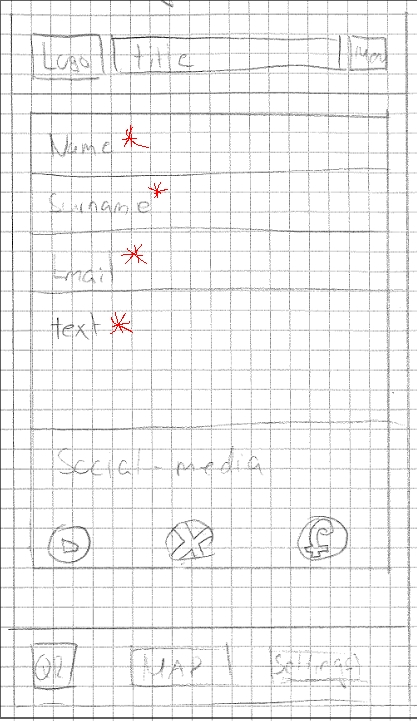
\includegraphics[width=5cm]{required-fields.jpg}
	\subsubsection{Eingabeformate}
	Falls sich der Benutzer im Internet nicht auskennt, kann es verwirrend sein, was bei den Feldern erwartet wird. Deshalb muss das klar erkennbar sein.\\
	Ich denke, dass es am einfachsten verständlich ist, wenn man einen Passenden Platzhalter für jedes Feld macht. Dabei soll der Platzhaltertext gräulich sein, damit man erkennt, dass es nicht Text ist, der wirklich ins Eingabefeld geschrieben ist.\\
	Als Platzhalter würde ich eine mögliche Eingabe nehmen. Beim Email Feld könnte das z.\,B. \textit{max.mustermann@example.com} sein.
	\subsubsection{Felder im Detail}
	Den Namen würde ich mit einem roten Stern kennzeichnen. Als Platzhalter würde ich Mustermann nehmen.\\
	Beim Feld für den Vornamen würde ich auch einen Stern platzieren. Statt Mustermann würde ich dann Max verwenden.\\
	Das Email Feld habe ich oben schon als Beispiel verwendet. Dieses würde ich auch mit einem Stern markieren und wie schon gesagt als Platzhalter \textit{max.mustermann@example.com} verwenden.\\
	Für den Text (die Nachricht) würde ich auch einen Stern verwenden. Als Platzhalter würde ich «\textit{Ihre Nachricht hier}» verwenden.
	
	\pagebreak
	
	\subsection{Hilfe und Feedback integrieren}
	
	\subsubsection{Feedback für User aktionen}
	
	Ziel: User informieren dass die Anwendung auf ihren Input reagiert.
	
	\begin{itemize}
		\item Erfolgs Nachricht
		\subitem Nach Formular abgabe
		\subsubitem "Deine Änderungen wurden gespeichert"
		\subsubitem \textit{(Bestätigung der erfolgreichen Verarbeitung von Nutzereingaben)}
		\item Fehlermeldungen
		\subitem Fehlende Felder in Formular
		\subsubitem "Bitte fülle alle mit einem * Markierten Felder aus"
		\subsubitem \textit{(Klare Kennzeichung von Pflichtfeldern gemäss ISO 9241-110)}
		\subitem E-Mail Validierung fehlgeschlagen
		\subsubitem "Invalides E-Mail Format. Beispiel: user@example.com"
		\subsubitem \textit{(Formatvorlge zur sofortigen Fehlerbehebung)}
		\item Ladeanzeiger / Animationen
		\subitem Datenabfragen
		\subsubitem Loading Spinner / Wheel
		\subsubitem \textit{(Visuelles Feedback bei kurzen Wartezeiten <3s)}
		\subitem File upload
		\subsubitem Progress Bar
		\subsubitem \textit{(Prozentuale Anzeige für längere Prozesse)}
		\subitem Kontent Ladescreen
		\subsubitem Skellet-Screen (normaler screen ohne Daten)
		\subsubitem \textit{(Wahrung des Aussehens und Format während des Ladens)}
	\end{itemize}
	
	Wir haben uns hier dafür entschieden eine Erfrolgsnachricht anzuzeigen wenn das Kontakt Formular abgesendet wird, die Felder Validierung einzu arbeiten und beim ersten starten der App eine Progressbar damit der User weiss wie schnell die Daten runter geladen werden.
	
	\subsubsection{Hilfefunktionen}
	
	Ziel: Benutzer unterstützen, falls sie unsicher sind, wie das Kontaktformular ausgefüllt werden soll.
	
	\begin{itemize}
		\item Platzhaltertext in Eingabefeldern
		\subitem Beispiel für das "Name"-Feld:
		\subsubitem \texttt{"Max Mustermann"}
		\subitem Beispiel für das "Betreff"-Feld:
		\subsubitem \texttt{"Betreff meiner Nachricht"}
		\subsubitem \textit{(Führt den Nutzer durch implizite Beispiele)}
		
		\item Automatische Vorschläge
		\subitem Bei der "E-Mail"-Eingabe:
		\subsubitem \texttt{"Meinten Sie: example@domain.com?"}
		\subsubitem \textit{(Typos erkennen durch Domain-Check)}
	\end{itemize}
	
	Wir werden hier beides implementieren um die UX der User zu verbessern.
	
	\subsubsection{Erweitertes Feedback}
	
	Ziel: Für eine Polierte UI, um Hilfe und Feedback dynamisch zu kombinieren.
	
	\begin{itemize} 
		\item Real-time validation
		\subitem zBs. Passwort Stärke Messer
		\item Rückgänig machen Option
		\subitem zBs. Wenn man eine Formular Sende Bestätigung bekommt, das man diese inerhalb von 5s noch zurück ziehen kann.
		\item Interaktives Tutorial
		\subitem zBs. Ein Step-by-step popup für neue Nutzer
	\end{itemize}
	
	Auch hier würden wir alles implementieren da es für die Nutzer die beste experience gibt.
	
	\pagebreak
	
		\section{Band C}
	\subsection{Elemente einer Benutzerschnittstelle kennen und anwenden}
	\subsubsection{Controls und Widgets erklären}
	\subsubsubsection{Was sind controls und Widgets}
	Controls oder Widgets sind grafische Steuerelemente einer Benutzeroberfläche. Sie ermöglichen dem Benutzer, mit einem Programm zu interagieren, Eingaben zu machen und Informationen zu erhalten. Controls und Widgets sind nicht alle Interaktionselemente, da mache nur für die datenübergabe an den Nutzer sind.
	
	\subsubsubsection{Häufig verwendete Controls und Widgets}
	\begin{tabular}{@{}lll@{}}
		\toprule
		\textbf{Widget / Control} & \textbf{Beschreibung} & \textbf{Wichtige Eigenschaften} \\
		\midrule
		Button (Schaltfläche) & Ein klickbares Element, das eine Aktion auslöst. & Text, Icon, aktiv/deaktiviert \\
		Label (Beschriftung) & Zeigt Text oder Information an, keine Interaktion. & Text, Schriftart, Ausrichtung \\
		Textfeld (Textbox) & Ermöglicht die Eingabe von Text durch den Benutzer. & Inhalt, Länge, Passwortmodus, aktiv/deaktiviert \\
		Checkbox (Kontrollkästchen) & Ermöglicht das An- oder Abwählen einer Option. & An/Aus-Zustand \\
		Radiobutton (Optionsfeld) & Ermöglicht das Auswählen einer Option aus einer Gruppe. & Gruppenzugehörigkeit, Auswahlstatus \\
		Dropdown (Auswahlliste) & Ermöglicht die Auswahl eines Werts aus einer Liste. & Ausgewählter Wert, Listeneinträge \\
		Slider (Schieberegler) & Ermöglicht das Einstellen eines Werts innerhalb eines Bereichs. & Minimalwert, Maximalwert, aktueller Wert \\
		Progressbar (Fortschrittsanzeige) & Zeigt den Fortschritt eines Vorgangs an. & Minimalwert, Maximalwert, aktueller Wert \\
		Image (Bild) & Zeigt ein Bild oder Icon an. & Dateipfad, Größe, Skalierung \\
		\bottomrule
	\end{tabular}
	
	\subsubsection{Controls und Widgets sinvoll verwenden}
	\subsubsubsection{was bedeutet sinvoll plaziert}
	Sinvoll plazierte Widgets und Controlls sorgen dafür das der Nutzer die Seite möglichst Intuitive und Effizient navigieren kann. Unteranderem sollten einfach erkenbare Symbole verwendet werden und diese sollte an den gewohnten stellen plaziert sein. Wenn ein User nach etwas sucht, dann sollte er ohne lange suchen zu müssen fündig werden.\\
	Wir haben unsere Symbole und die Plazierung der Element, vor allem in der Nav bar, von der SRF Webseite inspirieren lassen, da diese Seite stark besucht ist und damit unsere Applikation unseren Usern schon bekannt vor kommen sollte.
	\\
	\subsubsubsection{Sinvolle Umsetzung}
	In userer Umsetzung haben wir die ERlernte Theorie angewendet. Die Navbar und die Suchfunktion ist wie bei SRF und sollte den meisten Kunden bereits bekannt vorkommen.
	\\
	Der Hauptinhalt der Seite ist die Interaktive Karte.
	\\
	Unsere Footer Bar besteht aus 3 gängigen Symbolen.
	\begin{itemize}
		\item QR-Code
		\item Map
		\item Einstellungszahnrad
	\end{itemize}
	Das sind alles sehr gängige Symbole welche für fast jeden sofort verständlich sein sollten.\\\\
	Unsere Search funktion ist auch auf SRF basiert und ist so Intuitive wie möglich gestalltet. Alle möglichen Aktionen sind sofort Zentral ersichtlich. Der hintergrund wird aus dem Fokus genommen damit die neuen Interaktionsmöglichkeiten herausstechen und die zuvor besuchte Seite immer noch so halb ersichtlich ist, dies sollte sicherstellen das die Nutzer wissen das die vorherige Seite nicht verloren gegangen ist.\\\\
	Die Settingspage ist bekannten überkategorien organisiert mit der Accessibility ganz oben damit man schnell den Screenreader oder die Schriftgrösse zu seinen präferenzen ändern kann.<
	\\
	\subsubsection{Controls und Widgets in eine Logische abfolge bringen}
	Durch Umfgragen mit mehreren Dritten personen und Inspirationen von verschiedenen Webseiten haben wir die Plazierung und die Zusammenareit unserer Controlls und Widgets Optimiert. Wir haben unseren Fokus auch auf einen Logischen Aufbau gelegt damit es für jeden, auch für Kinder oder Ältere personen, einfach verstehen können. Unsere Applikation ist jetzt sehr intuitive und sollte für jeden brauchbar sein.
	\\
	
	\subsection{Benutzerschnittstelle erstellen und testen}
	\subsubsection{Skitzen als Prototyp umsetzen}
	Ich habe micht dazu entschieden, den Prototypen als Webseite zu bauen. Bei der Arbeit entwickle ich auch Webseiten. Deshalb geht das für mich einfacher, als ein neues Tool zu lernen. Wenn wir dann die richtige App programmieren würden, könnten wir auch den Code aus dem Prototypen weiter verwenden.\\
	Hier ist der Link zur \href{https://davidhafner.github.io/M322-Documentation/}{Webseite}\\\\
	
	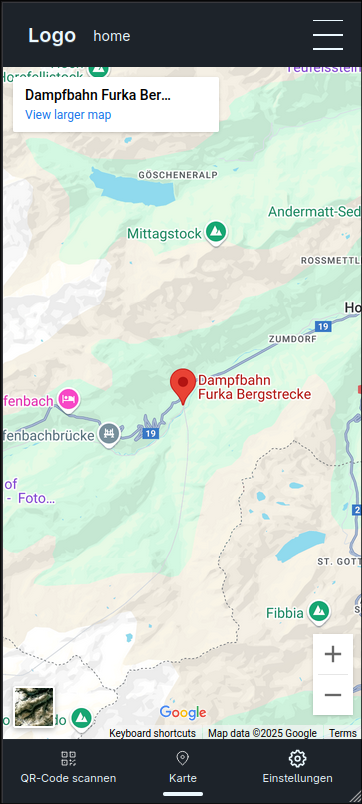
\includegraphics[width=7cm ]{mainpage}
	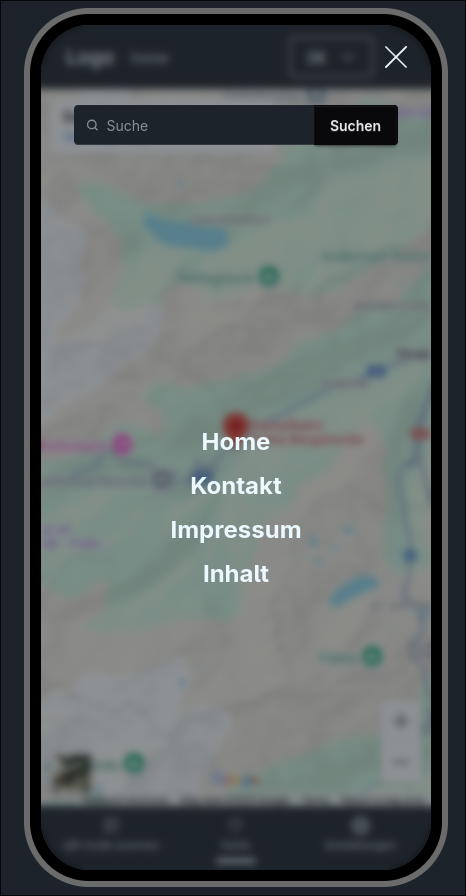
\includegraphics[width=7cm ]{searchpage}
	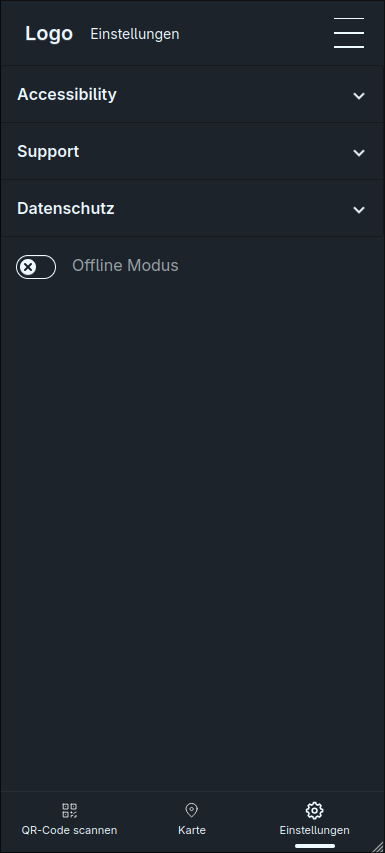
\includegraphics[width=7cm]{settingspage}
	\\\\
	\subsubsection{Testen und Probleme indentifizieren}
	\begin{itemize}
		\item Den Prototypen habe ich nur für die Mobile ansicht optimiert. Im Desktopmodus sieht er nicht so gut aus.
		\item Wenn man mit dem Menu von einer Seite zu einer anderen wechselt bleibt das Menu offen. Das ist nicht intuitiv.
		\item Da ich im Browser den Dark mode verwende, sieht sie im light mode nicht so gut aus.
	\end{itemize}
	\subsubsection{Verbesserungen}
	\begin{itemize}
		\item Da der Prototyp nur für Mobile optimiert sein muss, könnte ich es auf grossen Bildschirmen in ein Handy packen. So kann man die Webseite trotzdem gut testen.
		\item Wenn im Menu eine Seite gewählt wird, werde ich machen, dass das Menu automatisch schliesst.
		\item Ich werde die Webseite im light mode testen.
	\end{itemize}
	
	
	
	
	\subsection{Benutzerfreundlichkeit verbessern}
	\subsubsection{Schwierig unzusetzende Elemente}
	\begin{itemize}
		\item 	Dropdown schließt nicht automatisch bei Klick außerhalb
		\item 	Fehlende Keyboard-Navigation (Tab, Pfeiltasten, Enter)
		\item 	Schwierige Positionierung bei unterschiedlichen Bildschirmgrößen
		\item 	Fehlende Barrierefreiheit (ARIA-Rollen und Attribute)
		\item 	Probleme bei responsivem Verhalten auf kleinen Bildschirmen
		\item 	Unklare oder zu kleine Klickflächen
		\item 	Schwierige State-Verwaltung (Öffnen/Schließen, Selektion)
	\end{itemize}
	Wir haben uns entschieden spezifisch die folgenden Punkte zu berücksichtigen.
	\begin{itemize}
		\item 	Schwierige Positionierung bei unterschiedlichen Bildschirmgrößen
		\item 	Probleme bei responsivem Verhalten auf kleinen Bildschirmen
		\item 	Unklare oder zu kleine Klickflächen
	\end{itemize}
	
	\subsubsection{Verbesserungen Unterbreiten}
	Als Verbesserung werden wir anstadt unsere Buttons Anzuschreiben Symbole verwenden. Dies sollte gut die Grösse des Buttons Klar.\\
	Die Applikation werden wir auch kommplet dynamisch gestalten damit diese auf allen möglichen Bildschirmen Funktioniert.
	
	\subsubsection{Implementation}
	Diese Vorschläge haben wir in intuitive und einfachere Lösungen umgesetzt, was dazu beigetragen hat, dass sich die Nutzer:innen schneller zurechtfinden und sich das Design insgesamt runder und benutzerfreundlicher anfühlt. Besonders stolz sind wir darauf, dass diese Verbesserungen am Ende einer positiven Gesamtbewertung geführt haben
	
	\pagebreak
	
	\section{Band D}
	\subsection {Walktrough einer Benutzerschnittstelle}
	\subsubsection{Was ist ein Walktrough}
	Ein Walktrough ist eine begleitet führung durch die applikation bei der die einzelnen Benutzerschnittstellen erklärt werden. Dies sollte den Testpersonen die Basics der Applikation erklären.
	\subsubsection{Walkthrough Durchführen}
	Als Testperson wird der Kleine Bruder einer der Teammitglieder Verwedet.\\\\
	Zuerst wird die Navbar erklärt und was alles damit gemacht werden kann. Durch die Intuitive gestaltung ist nicht viel erklärung notwendig. Weiter geht es zum Hautteil der Seite mit der Interaktiven Karte, da dies ein Platzhalter ist kann hier nicht viel gemacht werden. Zum schluss der Hauptseite wird der Footer und dessen einzelnen Seiten erklärt. Durch die Symbolnutzung ist das nicht aufwendig. In den Einstellungen werden dann die Verschiedenen möglichkeiten mit den Dropdowns vorgezeit mit einem Fokus auf die Accessability menu. Als letztes wird das Suchfeld erklärt. Testmässig wird auch noch ein Kontaktformular ausgefüllt.\\\\
	Damit ist der Kurze Walktrough der App fertig. Alle wichtigen Benutzerschnittstellen wurden vorgezeigt und können jetzt von der Testperson effizient verwendet werden.
	\subsubsection{Usability-Test}
	Ein Usability-Test ist ein Test bei dem einem Testuser eine Aufgabe gestellt wir dund dieser versucht dies in der Applikation umzusetzen. Bsp. Fülle ein Rückmeldeformular aus oder ändere die Schriftgrösse auf 200\%. Das sind alles Aufgaben welche die normalen Nutzer wärend der durchschnitlichen Nutzung der App abschliessen müssen.
	\subsubsubsection{Usability-Test durchführen}
	Für Unseren Usiability Test werden wir der Testperson 3 Aufgabe stellen welche der Durchschnittsuser bewältigen können muss.
	\begin{itemize}
		\item Die Schrifftgrösse auf 200\% stellen
		\item Die Eine Kontaktemail Schreiben
		\item Den QR-Code und das Suchfenster verwenden.
	\end{itemize}
	Der Usability-Test ist gut ausgefallen. Alle Aufgaben konnten inerhalb von Kürzester Zeit abgeschlossen werden ohne weiteren Input.\\
	Da der Tester die Applikation Problemlos navigieren konnte lässt sich daraus schliessen, das die Benutzerfreundlichketi eher hoch ist.\\
	Da alle Aufgaben schnell und mit minimalem aufwand abgeschlossen werden konnten, kann man auch daraus schliessen das die Effizeinz der Applikaion auch eher hoch ist.
	\\\\
	Als Kommentar zu Unserer Applikation gab einer der Testpersonen an, die Applikation sei "sehr Sigma".
	\subsection{Usability quantifizieren undverbessern}
	Reflexion zur Usability-Überprüfung
	Für die Bewertung der Benutzerfreundlichkeit unseres Prototyps habe ich einen standardisierten Fragebogen benutzt. Die Rückmeldungen der Testperson habe ich anschliessend ausgewertet und mit einer Nachbefragung vertieft (Gespräch, weshalb sie dieses Feedback gegeben hat). Dabei kamen konkrete Verbesserungsvorschläge zusammen, zum Beispiel, dass sich das Menü automatisch schliessen sollte, wenn man einen Menü-Punkt auswählt
	Diese Rückmeldungen haben wir fast alle direkt umgesetzt. Trotzdem zeigte die Auswertung, dass sich die Nutzererfahrung verbessert hat. Die meisten fanden das Design ansprechend und die Navigation einfach.
	Abschliessend habe ich die gesammelten Daten analysiert und daraus konkrete Verbesserungsschritte abgeleitet. Ich finde, dass wir durch diesen Prozess ein gutes Verständnis dafür entwickelt haben, wie man Benutzererfahrung misst und sinnvoll optimiert und dass schon kleine Änderungen einen grossen Unterschied machen können.
	
	\pagebreak
	
	\section{Band E}
	\subsection{Barrierefreiheit umsetzen}
	\subsubsection{Was ist barrierefreiheit in einer Applikation}
	Barrierefreiheit beschreibt wie einfach die Applikation gebraucht werden kann auch für personen mit einschränkungen.
	Einige Beispiele von Barrierefreiheit sind:
	\begin{itemize}
		\item Screenreader
		Eine Möglichkeit den inhalt der Applikation vorgelesen bekommen zu können. Ideal für Blinde Nutzer.
		\item Schriftgrösse verstellen
		Die verstellung der schrifftgrösse erlaubt es auch Personen mit Seheinschränkungen die Applikation problemlos zu verwenden.
		\item Einfache Sprache
		Die Sprache in der Applikation sollte simpel gehalten werden das auch junge Personen oder Personen welche sich nicht im Fachbereich auskennen den Inhalt trotzdem verstehen können.
		\item Sprachen
		Mehrere Sprachen erlauben es mehr verschiedenen Nutzer die Applikation zu verwenden.
		\item Symbole
		Symbole verwenden damit alle möglichen Personen möglichst schnell die Funktion eines Knopfes verstehen können\\\\
	\end{itemize}
	
	Beim entwerfen einer Applikation sollte auf die Barrierefreiheit geachtet werden, aber die Anforderungen sind nicht für alle gleich. Für eine Applikation mit der man sich für eine schwiereige English Prüfung anmelden kann, braucht nicht mehrere Sprachoptionen.\\
	Oder bei der Webseite für einen Augenoptiker lohnt es sich eine leicht verstellbare schriftgrösse zu haben.
	\subsubsection{Barrierefreiheit unserer der Applikation}
	Da unsere Applikation von alle möglichen Personen verwendet werden kann. Es sollte also simple Sprache verwenden, eine verstellbare Schriftgrösse haben und zusätzlich noch einen Screenreader haben.\\ Dies haben wir alles in den Einstellungen als Option angegeben.\\
	Die möglichkeit schnell zwischen allen 4 gängigen Landessprachen zu wechseln ist in der Navbar aufzufindne.
	Fast alles wird mit Symbolen beschrieben. Alles wird somit Intuitive gestaltet und erlaubt damit dass alle unsere App problemlos verwenden können.
	
	\subsection{Barrierefreiheit prüfen}
	\subsubsection{Wie kann Barrierefreiheit Prüfen}
	Zum Prüfen von Barrierfreihiet in Applikationen gibt es mehrere möglichkeiten.
	\begin{itemize}
		\item Automatische Tools
		\item Checklisten mit Richtlinien
		\item Nutzertest
		\item Manuelle Tests
	\end{itemize}
	Da wir keine Nutzer haben, Die Onlinetools nicht immer alles erwichen und wir keine Zeit haben alles Manuell zu testen, haben wir uns für die Checkliste mit Richtlinein entschieden.
	\subsubsection{Barrierefreiheit-Checklist}
	Aus den Rahmenbedingungen der Applikation konnten dies Checkpunkte für die Barrierefreihet herausgelesen werden.
	\begin{itemize}
		\item Alle 4 Landessprachen sollten verfügbar sein
		\item Gut Lesbare Schrift
		\item Screenreader für Seheingeschränkte
		\item Verstellbare Schriftgrösse
		\item Simple Sprache
	\end{itemize}
	\subsubsection{Benutzerschnittstelle gemäss checkliste Prüfen}
	Als Benutzerschnittstell nehmen wir die Hauptseite.
	\begin{itemize}
		\item Es gibt die möglichkeit schnell von hier zwischen den Landessprachen zu wechseln.
		\item Die Schrifft welche verwendet wird ist gut lesbar, der Rest ist mit leicht verständlichen Symbolen gestaltet.
		\item Der Screenreader ist über die Einstellungen verfügbaer und ist Standardmässig eingeschaltet
		\item Die Schriftgrösse ist über die  Einstellungen verstellbar
		\item Der Text der verwendet wird ist Simple oder wird durch Symbole Klar gemacht
	\end{itemize}
	
	\subsubsection{Barrierefreiheit Nachweisen}
	Die Barrierefreihet wurde durch das testen mit mehreren Personen Nachgewiesen. Keiner der Testpersonen hatten Probleme beim verwenden oder verstehen der Applikation.\\\\
	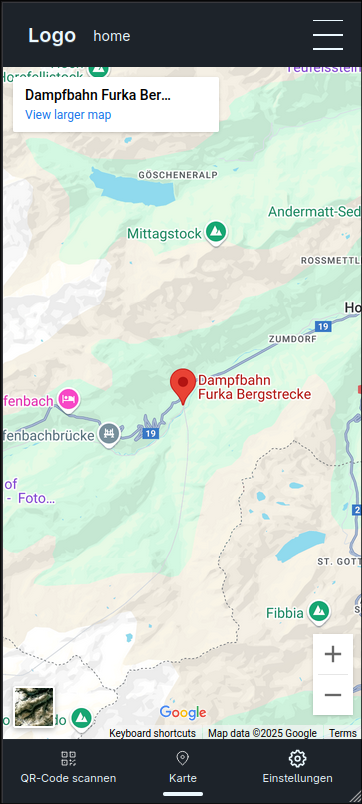
\includegraphics[width=7cm ]{mainpage}
	
\end{document}